%!TEX root = ..\..\dissertation.tex
\section{Classification Coding of Manufacturing Systems}\label{sec:PSCC}
\cref{paper:clsfCoding} is entitled~\citetitle{SorensenClsfCoding}, written for and submitted to a journal in 2018, currently undergoing a second round of review.
It relates to and addresses \cref{resq2} by answering the following sub-questions:
\begin{enumerate}[leftmargin=3em]
  \item[RQ2.2]What are the essential aspects of manufacturing systems that must be captured in order to classify them?
  \item[RQ2.3]What is the best form/structure of a coding scheme that captures and classifies essential manufacturing system aspects/characteristics?
\end{enumerate}
Taking a design science research approach, this study presents several new \gls{glos:artefact}s for describing manufacturing systems; their design, structure, processes, and enablers.
It does so through a classification coding scheme with several digits, each representing a unique aspect of a manufacturing system.
Using this classification coding scheme, manufacturers can ensure consistent and standardised descriptions of their manufacturing systems as lines of digits, uniquely identifying each manufacturing system and facilitating objective comparison of manufacturing systems across departments.
Consistent and objective comparison and analysis of manufacturing systems enables identification of commonality and a variety of other characteristics and implications of design choices, that are not immediately obvious and can be beneficial to manufacturers.

\subsection{Extended Abstract}
\subsubsection*{Introduction}
Manufacturing systems have continuously evolved since their introduction during the first industrial revolution.
Changes in demand, technology, materials, and strategy keep pushing manufacturing systems forward in the search for improved performance and profits.
With the increasing performance of computing and sensing technology, data and advanced analytics are becoming available to manufacturers, facilitating timely decisions on when and which changes to make in manufacturing systems, thus enabling reconfigurable and changeable manufacturing~\parencite{ElMaraghySmartChange}.
Manufacturing systems capable of accommodating change (\ie{} changeable manufacturing systems) are still difficult to design and implement, although concepts and approaches based on the co-existence of product and manufacturing system platforms are becoming more popular~\parencite{MichaelisJohannesson,ElMaraghy2015407,ABBAS201851}.
However, development of platforms is no trivial matter either~\parencite{BossenPbCd,Andersen2017179}.

A key early step in the development of \gls{glos:platform}s is the identification of which assets to standardise and include in the platform, \ie{} \gls{glos:platformCand}s.
Often, the primary source of platform candidates is the tacit knowledge and intuition of system experts who have years of experience designing, maintaining, or working with the system~\parencite{SorensenMCPC2017}.
This does lead to the identification of platform candidates, but the process could be improved with more objective decision support, helping system experts justify their decisions and identify platform candidates that would otherwise been missed.

\subsubsection*{Classification Systems \& Coding}
Commonality between products have long been used to identify assets to include in a platform or product family~\parencite{Thevenot2006,Fixson01062007,schuh2014}.
One approach to forming these families is through group technology and coding, an approach for classifying and grouping assets based on their properties and similarities, whatever these may be~\parencite{Shunk1985GT}.
Several coding schemes exist~\parencite{JUNG1991223}, with the OPITZ scheme~\parencite{doi:10.1080/00207547108929870} being one of the more widely known schemes for parts and components, but few such schemes exist for manufacturing systems~\parencite{ElMaraghy2006Complexity,elmaraghy2010classification,ELMARAGHY201451}.
Based on the results of group technology and coding, manufacturing can be rearranged to improve performance, \eg{} a reduction in material handling and work-in-progress.
Group and classification coding schemes are often customised to fit a specific company or industry in order to achieve the best possible results in terms of efficiency and benefits, contributing to the fact that no parts classification and coding scheme has been universally adopted yet~\parencite{GrooverFourthGlobal}.

Coding schemes are typically numeric, consisting of a string of digits, each with a number of potential values.
Each of these values have a distinct interpretation.
In hierarchical codes, the interpretation of a value depends on the value of preceding digits, while the values in chain codes can be interpreted independently of preceding digits.
Usually, chain codes will require more digits in order to contain the same information as a hierarchical code, but it will be easier to interpret~\parencite{GrooverFourthGlobal}.
Hybrid codes combine these two types of codes, allowing a more flexible, but also potentially complicated, coding scheme.
Regardless of its type, a completed code will only ever have one clear interpretation.

Identifying commonality between manufacturing systems require that these be described in a consistent manner, for instance through a classification scheme, taxonomy, or ontology.
\textcite{McCarthy_MfgClassification} created a dendogram classifying manufacturing systems based on their operational objectives and characteristics, with \textcite{McCarthy_Cladistics} later developing a cladogram of automotive manufacturing systems, capturing their history based on 54 attributes.
Manufacturing systems have also been classified according to their ability to make adjustments, \ie{} according to their \gls{glos:changeability}~\parencite{WIENDAHL2007783,ElMaraghy2013629}.
\textcite{SorensenCMS2018} presented a consolidated process classification scheme for classifying manufacturing systems according to the processes they perform.
\textcite{Agarwal1994} proposes a similar process classification, albeit limited to manufacturing processes, in their coding scheme for parts and components.
\textcite{JARVENPAA201887} use an ontology to model the capabilities of manufacturing equipment, with each piece of equipment having a number of assorted capabilities, interfaces, and variables used to describe that specific equipment.
These resources and capabilities could be linked to a product model through a process taxonomy~\parencite{BRUNOE2018592}.

Classification and coding systems were initially developed for manufactured components and parts.
No equivalent system existed for manufacturing systems until the manufacturing structural classification coding (SCC) by \textcite{ElMaraghy2006Complexity}.
It was introduced to classify equipment in a manufacturing system and the layout of these.
The SCC consists of two sub-codes---a layout classification code and an equipment classification code---with the equipment classification code itself capable of classifying three types of equipment; machines, transporters, and buffers.
While the first few digits of the equipment classification code vary depending on the equipment type, the remaining digits, describing control, programmability, and operation characteristics, are the same for all types of equipment.
The layout classification code describes the layout of the system, how it is controlled, programmed, and operated.
SCC is a chain code, with the value of each digit depending on the complexity of the corresponding entities; the higher the value, the higher the complexity.
Later, a classification coding scheme for assembly systems was developed by \textcite{elmaraghy2010classification}, extending the original SCC to include assembly-specific features and equipment. 
Both these classification codes are useful for comparing manufacturing systems and identifying commonality, as well as determining their complexity~\parencite{Samy2012}.

\subsubsection*{Method}
To structure development of the production system classification code (PSCC), \posscite{10.2307/25148625} information systems research framework was adopted.
With the framework's focus on development and justification of new \gls{glos:artefact}s---in this case, the sub-codes, digits, and their interpretations---it lends itself well to the development of a classification coding scheme.
Each digit must have an individual justification for existing in the coding scheme, they should address a specific need, be applied in an appropriate environment, and added to the growing knowledge base.
The iterative nature of the method and its internal design cycle were key to selection of the method and the design of the resulting coding scheme~\parencite{Hevner2007TheTC}.
New digits, values, and interpretations were suggested during each design cycle, and their justification for inclusion was evaluated based on the need and relevance of the knowledge they added to the coding scheme.
Several internal design cycles were carried out, followed by an application of the coding scheme to a number manufacturing systems.
This resulted in additional design cycles and an evaluation with an industrial partner.

In contrast to the aforementioned manufacturing and assembly system classification and coding schemes \parencite{ElMaraghy2006Complexity,Samy2012}, PSCC does not attempt to define nor calculate the complexity of systems, but does capture both physical (tangible) and logical (intangible) characteristics of manufacturing systems.
They capture \emph{why} and \emph{what} a system is, \emph{what} it does and \emph{how} it does it.
Certain digits in the coding scheme are inspired by and have been adopted from existing coding schemes, \ie{} they come from the knowledge base on manufacturing system and product coding.

\subsubsection*{Classification Coding Scheme}
An overview of the PSCC is shown on \cref{fig:PSCC_structure}.
\begin{figure}[tb]
  \centering
  \makebox[\textwidth][c]{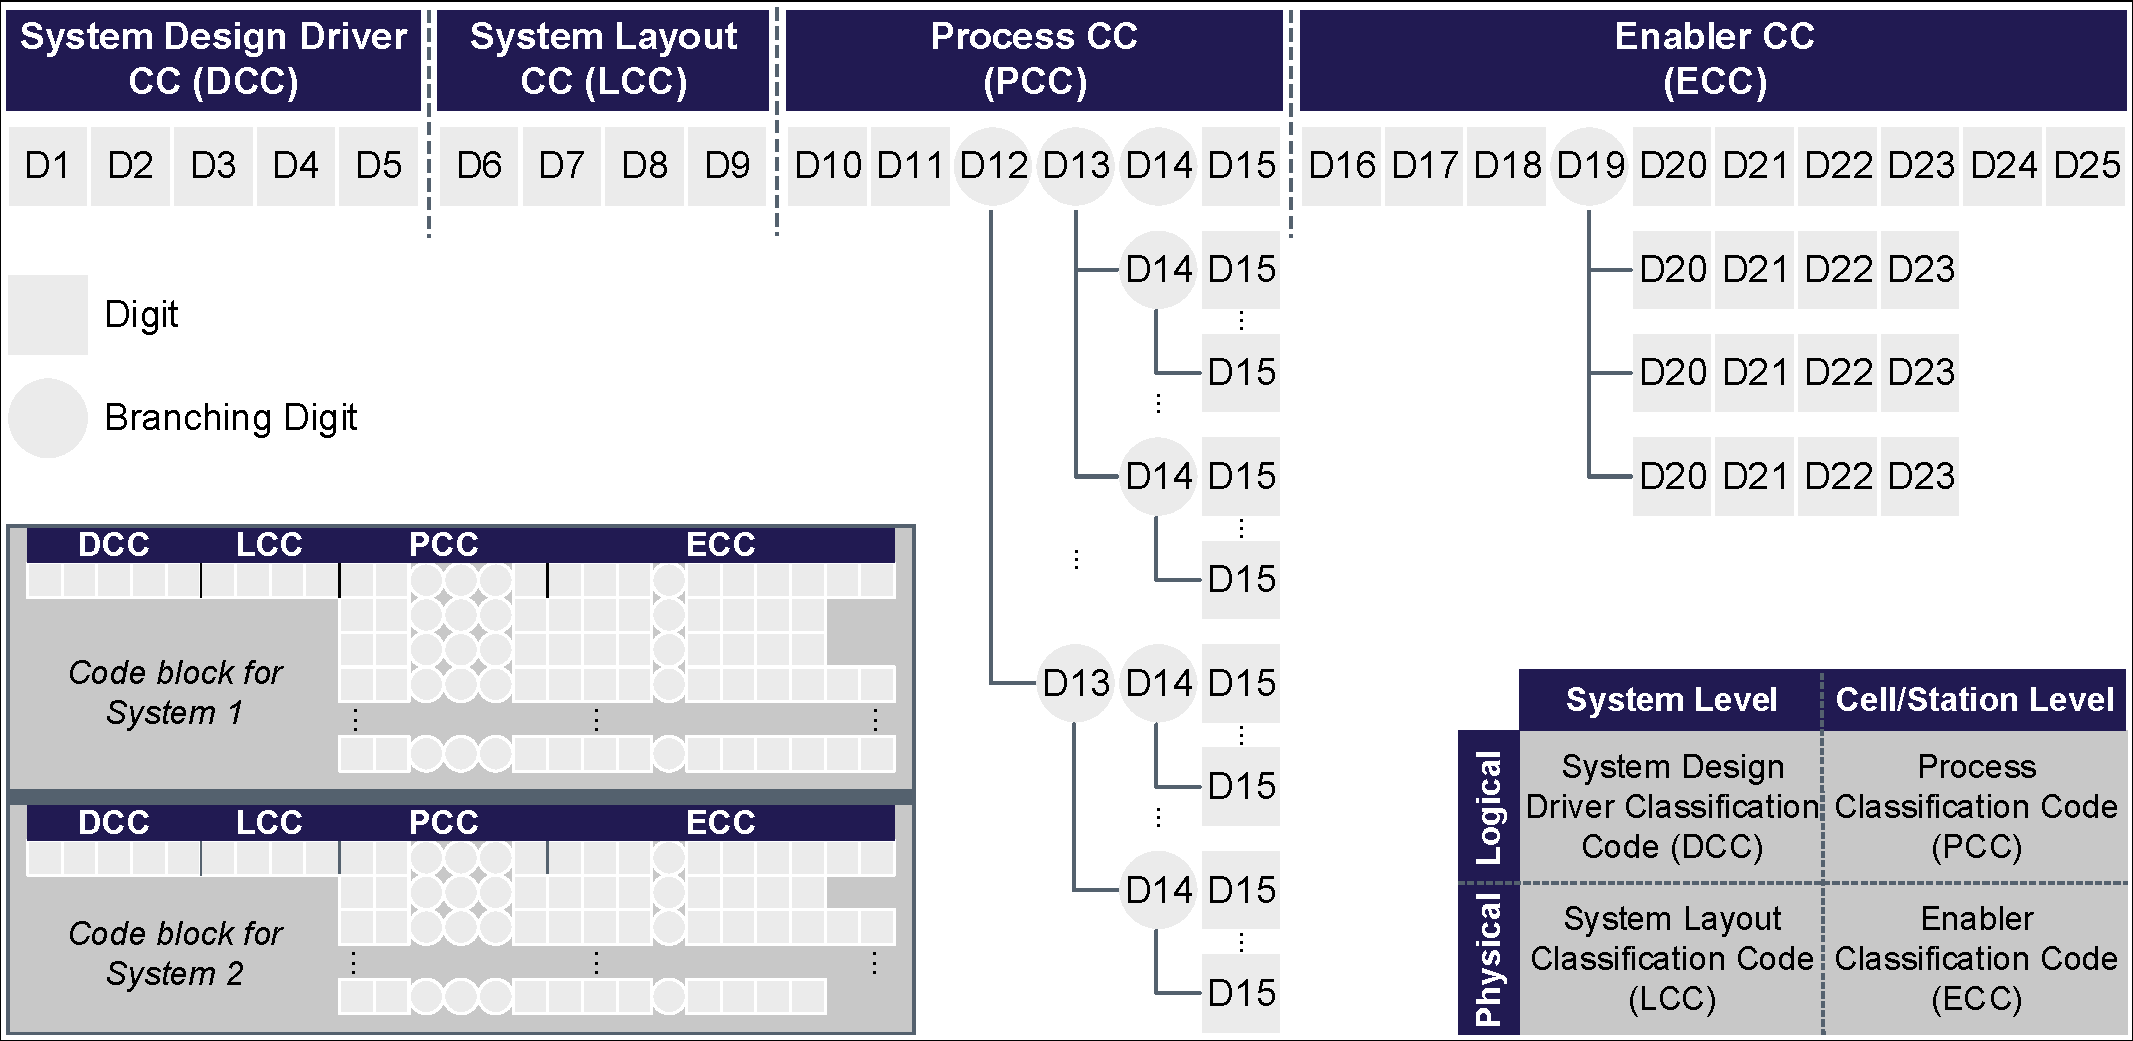
\includegraphics[width=1.1\textwidth, trim=3 3 3 3, clip]{mainmatter/researchResults/figures/PSCC_structure.pdf}}
  \caption[Structure and overview of the production system classification code (PSCC).]
  {Top: the structure of the production system classification code (PSCC).
  Bottom left: manufacturing systems described through blocks of code consisting of one DCC, one LCC and several PCC and ECC sub-codes.
  Bottom right: overview of the PSCC's four sub-codes.}\label{fig:PSCC_structure}
\end{figure}
It consists of four sub-codes (bottom right), each consisting of four to ten digits. 
These sub-codes describe and capture different aspects of the system-of-interest at various levels of abstraction.
Two sub-codes (system design driver classification code (DCC) and layout classification code (LCC)) are on a system level, and thus consider the manufacturing system as a whole.
The other two sub-codes (process classification code (PCC) and enabler classification code (ECC)) are on a cell/station level, and thus relate to individual elements of the manufacturing system.
DCC and PCC capture logical (intangible) characteristics of the system, while LCC and ECC capture physical (tangible) characteristics.
Physical characteristics are those that can be observed and collected directly from the system during observation, while logical characteristics require a deeper understanding of the system.
DCC (digits D1--D5) captures the rationale, reasoning, and drivers behind the design choices of a system, while the LCC (digits D6--D9) describes the layout of the system; PCC (D10--D15) captures all processes performed by the system, and ECC (D16--D25) describes the enablers carrying out the processes.
In this study, \emph{enabler} refers to the physical manufacturing equipment enabling production processes and the logical tools enabling planning and control of manufacturing systems.
The PSCC deals with the fundamental building blocks of manufacturing systems, the code strings being similar to biological DNA identifiers.
As such, it can be applied to any kind of manufacturing system, regardless of size, manufacturing paradigm, physical structure, or configuration.
\cref{tab:PSCC_DCC_SCC_PCC,tab:PSCC_ECC} elaborate on the 25 digits of the PSCC, providing a brief description of the characteristic captured by each.

\begin{table}[tb]
  \centering
  \caption[Digits and description for the DCC, SCC and PCC sub-codes in the PSCC.]
  {Digits and description for the DCC, SCC and PCC sub-codes in the PSCC~\parencite{SorensenClsfCoding}.}\label{tab:PSCC_DCC_SCC_PCC}
  \small
  \begin{tabular}{cll}
    \toprule
    \# & DCC & Description\\
    \midrule
    1 & Primary driver & Main reason for a specific system design.\\
    2 & Product size & Relative size of the manufactured product.\\
    3 & Production volume & Relative annual production volume.\\
    4 & Variety & Degree of variety of the manufactured products.\\
    5 & Paradigm & How the system accommodates change.\\
    \midrule
    \# & SCC & Description\\
    \midrule
    6 & Location & Physical, geographical location.\\
    7 & Shape & Physical shape of the system.\\
    8 & Automation & Overall level of automation.\\
    9 & Flow direction & Direction of material flow.\\
    \midrule
    \# & PCC & Description\\
    \midrule
    10 & Core & Core process are used on all manufactured variants.\\
    11 & Position & Position in sequence of processes.\\
    12 & Category & Process category.\\
    13 & Family & Decomposition of category.\\
    14 & Class & Decomposition of family.\\
    15 & Subclass & Decomposition of class.\\
    \bottomrule
  \end{tabular}
\end{table}
System design drivers captured in the DCC are the main reasons for a particular system's design, \eg{} product size, which drives the width of a conveyor, or production volume making manual processes infeasible.
These are typically documented in the system requirements or remain undocumented as tacit knowledge to system designers and experts.
This type of knowledge provides insight into why two seemingly similar systems have different physical instantiations.
Most of the digits in the DCC require customisation to the specific company.
The listed drivers are examples of common or generic drivers for system design.

Capturing the layout of the manufacturing system, the LCC captures physical characteristics unrelated to the operation of the system, but is more concerned with its location, shape, automation level, and material flow.
Location plays a part in determining an appropriate level of automation, depending on the specific country it is located in, and with a sufficiently detailed location parameter, it may directly influence design through floorspace or features that must be considered. 
Shape and flow is useful in describing the way material flows, and can be combined with the position digits (D10 and D16 in PCC and ECC respectively) to link layout, processes, and enablers, also capturing cases where two processes are carried out by the same enabler at different points in the overall process.

In the PCC, the processes carried out by the system are captured and classified according to a consolidated process classification scheme~\parencite{SorensenCMS2018}, but currently leaving out the control and planning processes.
It also captures the position of each process in the material flow, and notes whether a process is used for all variants manufactured by the system or only specific variants.
All of this can be used to better understand the function of a manufacturing system, and how the product is transformed through the system, with the position digit being useful in potentially generating process flow diagrams.

The ECC consist of five common digits (digits D16--D20), with digit D19 creating four branches of the sub-code; one for each type of enabler (machine, handling, buffer, or fixture).
For each enabler, a position, structure, sourcing, category, and type is needed to describe the enabler on a high level, tying it to a specific location on a production layout (via the position digit D16), and linking it to a specific process.
The three to five remaining digits describe the specific features of the enabler, so differences and similarities in their physical instantiations can be captured and analysed.
\begin{table}[tb]
  \centering
  \caption[Digits and description for the ECC sub-code in the PSCC.]
  {Digits and description for the ECC sub-code in the PSCC~\parencite{SorensenClsfCoding}.}\label{tab:PSCC_ECC}
  \small
  \begin{tabular}{cll}
    \toprule
    \# & ECC & Description\\
    \midrule
    16 & Position & Position in sequence of processes.\\
    17 & Structure & Degree to which the enabler accommodates change.\\
    18 & Sourcing & In-house or contracted design of enabler.\\
    19 & Category & Enabler category.\\
    20 & Type & Specifies enabler type based on category.\\
    \midrule
    \# & Machine ECC & Description\\
    \midrule
    21 & Spindles & Number of rotary axes moving parts/tools.\\
    22 & Work heads & Number of work heads carrying out operations.\\
    23 & Axes of Motion & Number of axes of motion enabler can move along.\\
    24 & Tools & Degree to which tools can be changed.\\
    25 & Fixture & Degree to which fixture can be changed.\\
    \midrule
    \# & Handling ECC & Description\\
    \midrule
    21 & Path & Degree to which path of enabler can be changed.\\
    22 & Power & Whether the enabler requires power to function.\\
    23 & Part Types & Capability to handle one or more part types.\\
    \midrule
    \# & Buffer ECC & Description\\
    \midrule
    21 & Access & Order in which parts are accessed by enablers using buffer.\\
    22 & Location & Relative location to enabler using buffer.\\
    23 & Part Types & Number of different parts stored by enabler.\\
    \midrule
    \# & Fixture ECC & Description\\
    \midrule
    21 & Key Contact Points & Number of key contact points between fixture and part.\\
    22 & Fixing method & How a part is fixed/held by fixture.\\
    23 & Part Types & Capability to handle one or more part types.\\
    \bottomrule%
  \end{tabular}
\end{table}

\subsubsection*{Case Study \& Applications}
To illustrate potential applications of the PSCC, a case study was conducted at a large Danish manufacturer of discrete products.
Nine manufacturing systems were selected, manufacturing products of the same type, but with various sizes and features.
One code-block was created for each manufacturing system, consisting of one DCC and LCC as well as 12--34 PCC and ECC.
This resulted in a total of 190 lines of the PSCC in an spreadsheet made for the case study.
Afterwards, the populated codes were visualised, analysed, and simple comparisons were made on the nine systems based on a few select digits.

%Results
A visualisation of an interactive dashboard in PowerBI is shown on \cref{fig:clsfVis} to summarise the results of the case study.
(A) shows a count of process subclasses across the nine systems (the bars) and how large a portion of the systems the process appears in (prevalence, yellow line).
(C) shows the split of manufacturing, material handling, and test \& inspection processes across the systems, while (D) lists enablers by type, how often they are used, for what, and in which systems.
(B) is a data slicer for filtering visualisations.
The visualisation on \cref{fig:clsfVis} uses only five code digits (D2: product size, D3: production volume, D12: process category, D15: process subclass, D20: enabler type) and a system identifier.
Based on these five digits alone, a multitude of analysis and visualisations of the scoped manufacturing systems can be made, with an increasing level of detail and additional analysis as more digits are considered.
For instance, the allocate process (creation of a partial quantity and movement of said quantity to a specific location) occurs over 50 times and across all nine systems, while the screwing process occurs 30 times but only in 55\% of the systems, with 13 of these instances occurring in a single system.
\begin{figure}[tb]
  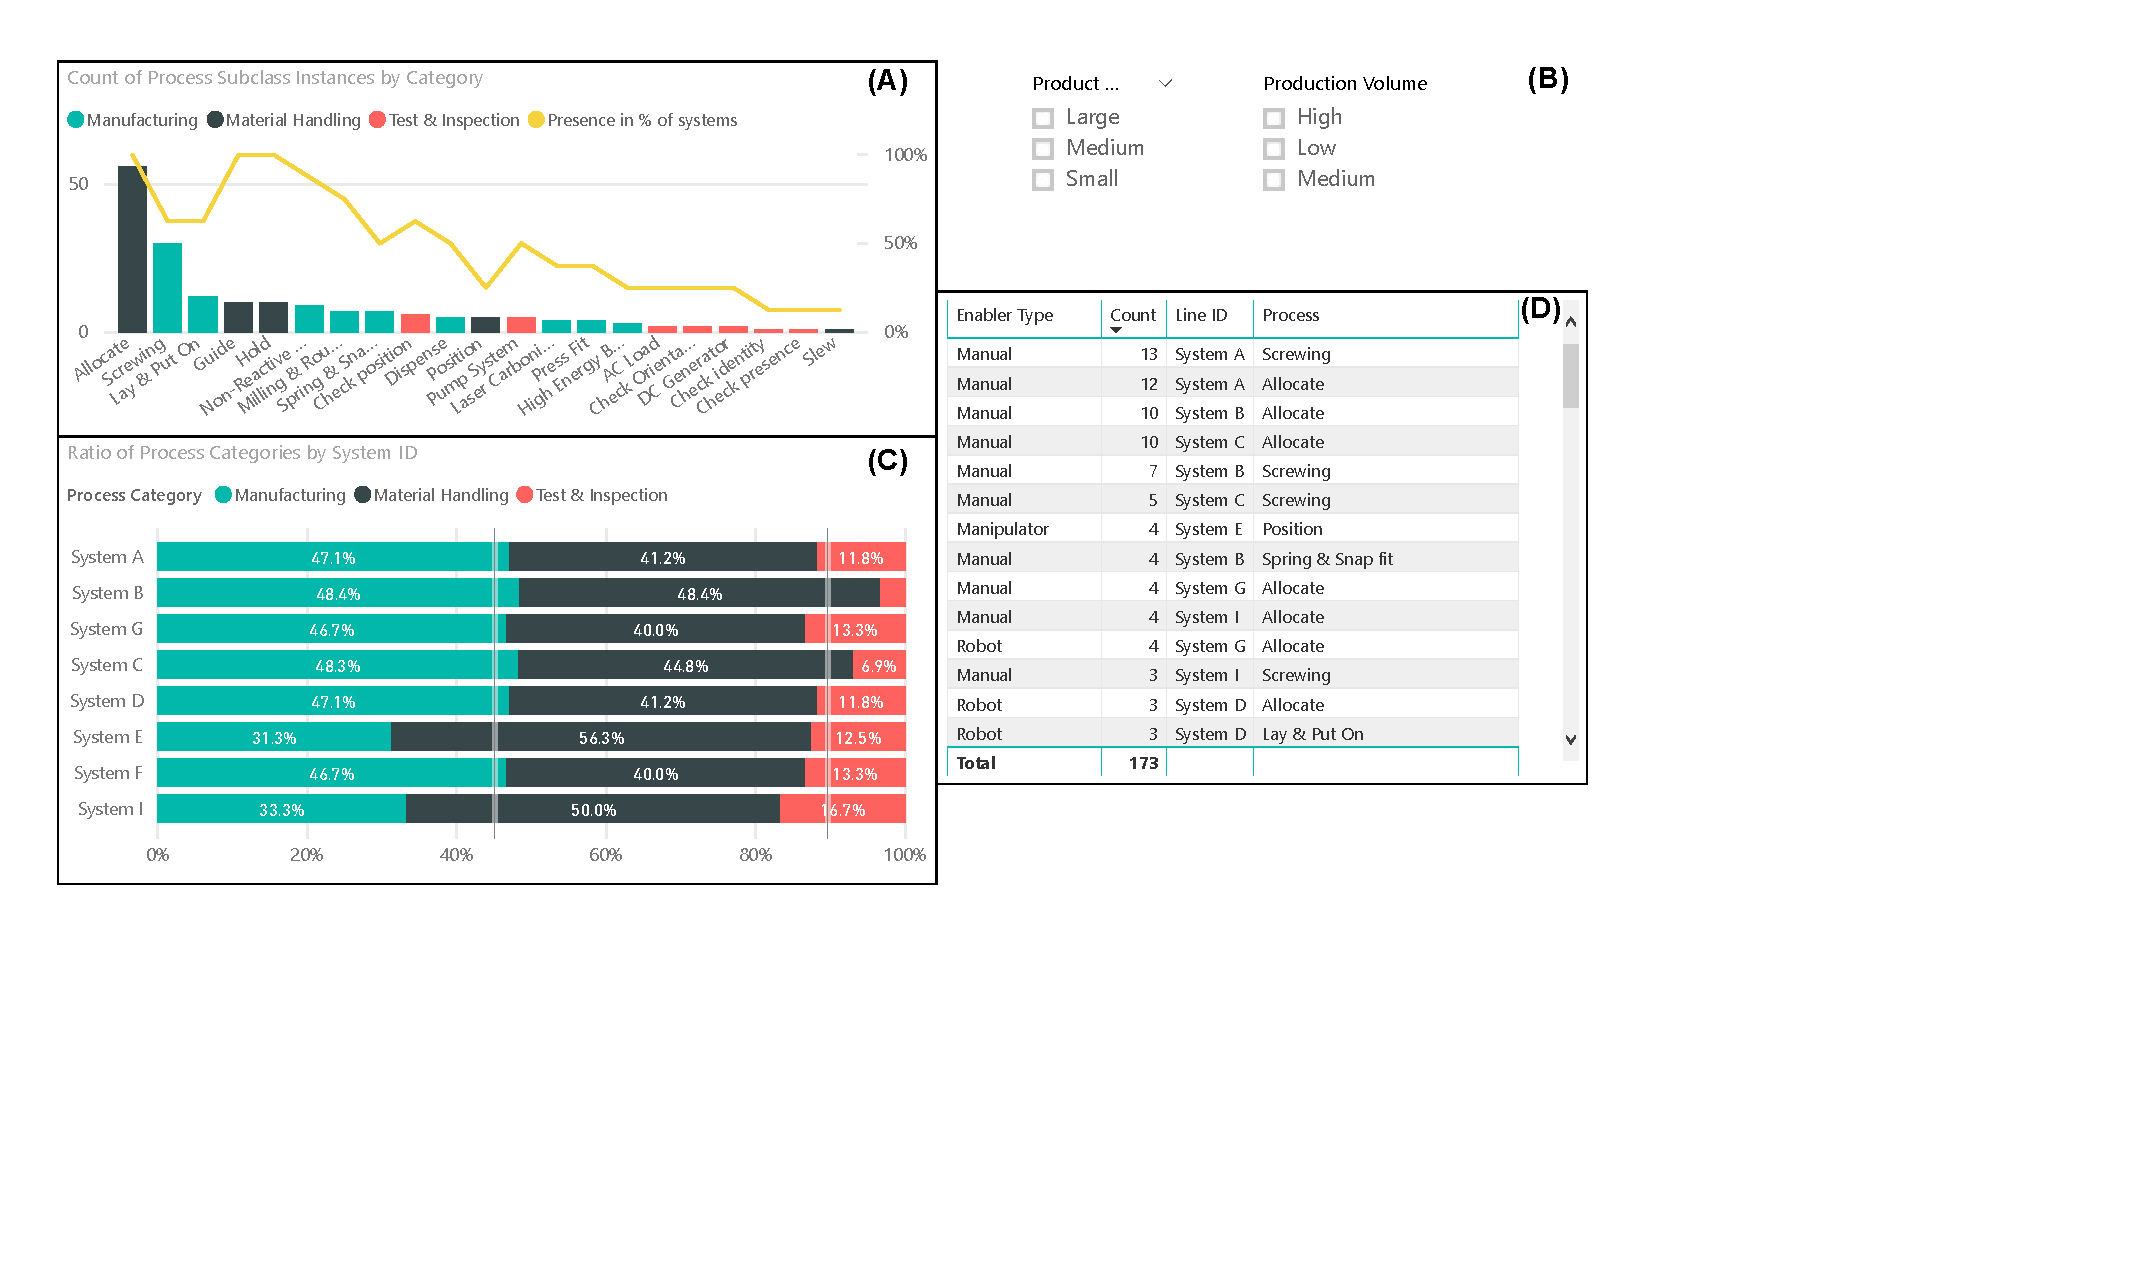
\includegraphics[width=\textwidth]{mainmatter/researchResults/figures/clsfVis.pdf}
  \caption[Example dashboard created from the populated code of nine manufacturing systems.]
  {Example interactive dashboard created from the populated code of nine manufacturing systems~\parencite{SorensenClsfCoding}.}\label{fig:clsfVis}
\end{figure}

%Applications
Using the code presented above, manufacturing systems can be compared to identify commonality.
It can help make the existing manufacturing capabilities and structure clear, so solutions can be reused for new purposes.
An algorithm can be applied to recommended specific platform candidates based on the company's requirements and the \gls{glos:cmmnlty} highlighted by the code.
Recommendations based on the code could be further strengthened by adding supplementary information on the manufacturing systems, such as their cost and performance.
This could also further enable a multitude of comparisons and analysis.
Simple and general comparisons between manufacturing systems can also be carried out, \eg{} based on D1--D9, providing a simple measure of similarity.
This measure, along with the recommendations for \gls{glos:platformCand}s, can be expanded with weighted factors and additional digits, allowing manufacturers to fine-tune the decision support tool according to their purposes and experiences.
Such measures can also be used to form manufacturing system families, providing benefits similar to product families, for instance by developing a solution for one system in a manufacturing system family and using it for other systems within the same family.

With its modular nature, the PSCC can also be used to capture and document the arrangement and connections of enablers, thus forming configurations~\parencite{HU2011715} that can be saved and used for future reference.
This can be beneficial both for design of new systems and reconfiguration of existing systems, as a database can be searched for previous or existing similar configurations, making use of any experience with these configurations.
It could also be used, alongside a modelling framework such as the one suggested by \textcite{BRUNOE2018592}, for determining the manufacturability of new products, and potentially suggesting changes or reconfigurations to the manufacturing system to improve manufacturability.

\subsubsection*{Conclusions}
The presented production systems classification code is intended to facilitate comparison of manufacturing systems within a manufacturing company, by standardising the manner in which these manufacturing systems are described, and outlining the data needed for this comparison.
It captures both physical and logical system characteristics on a system and cell/station level through a hybrid-code consisting of up to 25 digits grouped into four sub-codes, inspired by and incorporating digits from existing classification coding schemes.
The PSCC acts as a decision support tool, customisable and applicable to manufacturing systems regardless of the size of the company.
Even through analysis of relatively few systems and a partly populated code, the PSCC can provide value as shown during the case study, and with increased focus on big data and supplementary information such as performance and cost, the PSCC can be a powerful tool for a manufacturing company.
There are several potential applications outside the identification of platform candidates presented in this study, and the PSCC can be customised and expanded further to include more or different characteristics of manufacturing systems, including applications in the food, chemicals, and pharmaceuticals industry.

\subsection{Implications}
With development of the the production system classification code (PSCC) presented above, groundwork has been laid for standardising the description of manufacturing systems.
Their characteristics can be captured in a standardised format and subjected to numerous analysis providing value to various stakeholders within the company. 
It fills a gap within the case company itself, describing the structure and functions of their existing manufacturing systems, which has historically been missing.
This also enables manufacturers to link their standardised descriptions of manufacturing systems with their respective performance and cost data, providing valuable knowledge of their manufacturing systems across departments and factories.
For a manufacturer such as the case company, a manufacturing system \gls{glos:platform} represents a consolidation of their existing facilities and the definitive place to start when a new manufacturing development task is to be initiated.
In summation, the outcome of the study is:
\begin{enumerate}
  \item A classification coding scheme describing key aspects of manufacturing systems in a standardised format.
  \item Facilitation of an objective comparison of manufacturing systems across departments in a company.
  \item Groundwork enabling a variety of analysis approaches to determining why a system is performing well or poorly.
  \item A new classification coding scheme, numerous new digits, and experiences added to the knowledge base on classification coding and manufacturing system platform development.
\end{enumerate}